%% LyX 2.2.2 created this file.  For more info, see http://www.lyx.org/.
%% Do not edit unless you really know what you are doing.
\documentclass[english]{article}
\usepackage{courier}
\usepackage[T1]{fontenc}
\usepackage[latin9]{inputenc}
\usepackage{geometry}
\geometry{verbose,tmargin=0.8in,bmargin=0.8in,lmargin=1in,rmargin=1in,headheight=0cm,headsep=0cm}
\usepackage{babel}
\usepackage{array}
\usepackage{amsmath}
\usepackage{graphicx}
\usepackage[unicode=true,
 bookmarks=false,
 breaklinks=false,pdfborder={0 0 1},backref=section,colorlinks=false]
 {hyperref}

\makeatletter

%%%%%%%%%%%%%%%%%%%%%%%%%%%%%% LyX specific LaTeX commands.
\providecommand{\LyX}{\texorpdfstring%
  {L\kern-.1667em\lower.25em\hbox{Y}\kern-.125emX\@}
  {LyX}}
%% Because html converters don't know tabularnewline
\providecommand{\tabularnewline}{\\}

%%%%%%%%%%%%%%%%%%%%%%%%%%%%%% Textclass specific LaTeX commands.
\newenvironment{lyxcode}
{\par\begin{list}{}{
\setlength{\rightmargin}{\leftmargin}
\setlength{\listparindent}{0pt}% needed for AMS classes
\raggedright
\setlength{\itemsep}{0pt}
\setlength{\parsep}{0pt}
\normalfont\ttfamily}%
 \item[]}
{\end{list}}

%%%%%%%%%%%%%%%%%%%%%%%%%%%%%% User specified LaTeX commands.
\usepackage{babel}


\makeatother

\begin{document}

\title{CSCE 221 Cover Page\\
 Homework \#1 \\
 Due February 13 at midnight to eCampus}

\author{First Name~~Joseph ~~~~Last Name ~~Martinsen~~~~~~~~~~UIN~~323009961~~~}

\date{User Name ~~josephmart~~~~~~~E-mail address~~joseph@martinsen.com~~~~~\medskip{}
 }

\maketitle
 
\begin{quotation}
Please list all sources in the table below including web pages which
you used to solve or implement the current homework. If you fail to
cite sources you can get a lower number of points or even zero. According
to the University Regulations, Section 42, scholastic dishonesty are
including: acquiring answers from any unauthorized source, working
with another person when not specifically permitted, observing the
work of other students during any exam, providing answers when not
specifically authorized to do so, informing any person of the contents
of an exam prior to the exam, and failing to credit sources used.
Disciplinary actions range from grade penalties to expulsion read
more: \href{http://aggiehonor.tamu.edu/}{Aggie Honor System Office}\medskip{}
 \medskip{}
 
\end{quotation}
\begin{tabular}{|c|c|c|c|}
\hline 
Type of sources  & ~~~~~~~~~~~~~~~~~~~~~~~  & ~~~~~~~~~~~~~~~~~~~~~~~~  & ~~~~~~~~~~~~~~~~~~~~~~~\tabularnewline
 &  &  & \tabularnewline
\hline 
\hline 
People  &  &  & \tabularnewline
 &  &  & \tabularnewline
\hline 
Web pages (provide URL)  &  &  & \tabularnewline
 &  &  & \tabularnewline
\hline 
Printed material  &  &  & \tabularnewline
 &  &  & \tabularnewline
\hline 
Other Sources  &  &  & \tabularnewline
 &  &  & \tabularnewline
\hline 
\end{tabular}

\date{\medskip{}
 \medskip{}
 }

 
\begin{quotation}
I certify that I have listed all the sources that I used to develop
the solutions/codes to the submitted work.

``On my honor as an Aggie, I have neither given nor received any
unauthorized help on this academic work.\textquotedblright{} 
\end{quotation}

\date{\bigskip{}
 \bigskip{}
 }

\begin{tabular}{cccccc}
Your Name  & ~~~Joseph Martinsen~~~~~~~~  &  & ~~~~~~~~~~~~~~~~~~~~~  & Date  & ~~~02/11/2017~~~~~~~\tabularnewline
\end{tabular}\newpage{} 
\begin{quote}
\textbf{Type the solutions to the homework problems listed below using
preferably \LyX{}/\LaTeX{} word processors, see the class webpage
for more information about their installation and tutorial. } 
\end{quote}
\begin{enumerate}
\item (10 points) Write a C++ program to implement the Binary Search algorithm
for searching a target element in a sorted vector. Your program should
keep track of the number of comparisons used to find the target. 
\begin{enumerate}
\item (5 points) To ensure the correctness of the algorithm the input data
should be sorted in ascending or descending order. An exception should
be thrown when an input vector is unsorted.
\item (10 points) Test your program using vectors populated with consecutive
(increasing or decreasing) integers in the ranges from 1 to powers
of 2, that is, to these numbers:\\
 $1,\,2,\,4,\,8,\,16,\,32,\,64,\,128,\,256,\,512,\,1024,\,2048$.
\\
 Select the target as the last integer in the vector. 
\item (5 points) Tabulate the number of comparisons to find the target in
each range.

\begin{tabular}{|>{\centering}p{2cm}|c|c|c|c|c|}
\hline 
Range {[}1,$n${]}  & \multicolumn{1}{>{\centering}p{2cm}|}{Target for incr. values} & \multicolumn{1}{>{\centering}p{2cm}|}{\# comp. for incr. values} & \multicolumn{1}{>{\centering}p{2cm}|}{Target for decr. values} & \multicolumn{1}{>{\centering}p{2cm}|}{\# comp. for decr. values} & \multicolumn{1}{>{\centering}p{2cm}|}{Result of the formula in item 5}\tabularnewline
\hline 
\hline 
{[}1,1{]}  & 1  & 1  & 1  & 1  & 1\tabularnewline
\hline 
{[}1,2{]}  & 2  & 3  & 1  & 3  & 3\tabularnewline
\hline 
{[}1,4{]}  & 4  & 5  & 1  & 5  & 5\tabularnewline
\hline 
{[}1,8{]}  & 8  & 7  & 1  & 7  & 7\tabularnewline
\hline 
{[}1,16{]}  & 16  & 9  & 1  & 9  & 9\tabularnewline
\hline 
{[}1,32{]}  & 32  & 11  & 1  & 11  & 11\tabularnewline
\hline 
{[}1,64{]}  & 64  & 13  & 1  & 13  & 13\tabularnewline
\hline 
{[}1,128{]}  & 128  & 15  & 1  & 15  & 15\tabularnewline
\hline 
{[}1,256{]}  & 256  & 17  & 1  & 17  & 17\tabularnewline
\hline 
{[}1,512{]}  & 512  & 19  & 1  & 19  & 19\tabularnewline
\hline 
{[}1,1024{]}  & 1024  & 21  & 1  & 21  & 21\tabularnewline
\hline 
{[}1,2048{]}  & 2048  & 23  & 1  & 23  & 23\tabularnewline
\hline 
\end{tabular}

\newpage{}
\item (5 points) Plot the number of comparisons to find a target where the
vector size $n=2^{k}$, $k=1,2,\dots,11$ in each increasing/decreasing
case. You can use any graphical package (including a spreadsheet).

\begin{figure}[h!]
\centering{}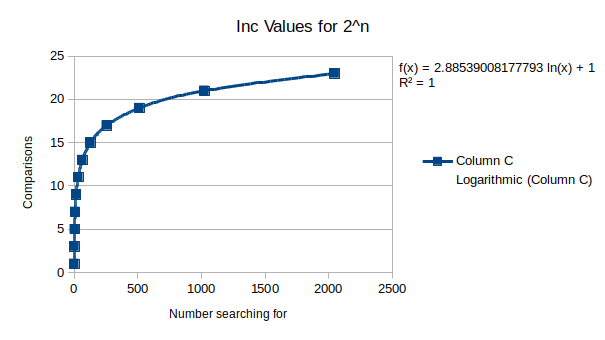
\includegraphics{inceven} \caption{Plot for Increasing/Decreasing Even Numbers}
\label{fig:1} 
\end{figure}

\item (5 points) Provide a mathematical formula/function which takes $n$
as an argument, where $n$ is the vector size and returns as its value
the number of comparisons. Does your formula match the computed output
for a given input? Justify your answer. \\

The equation for the best fit line of the graph is 
\begin{equation}
f(x)=2.88539\ln(x)+1
\end{equation}
The result is of plugging in the values to this equation is located
in the first table. The numbers are going to be nearly identical to
the number of comparisons due to the mean $R^{2}$ value being 1\\

\item (5 points) How can you modify your formula/function if the largest
number in a vector is not an exact power of two? Test your program
using input in ranges from $1$ to $2^{k}-1,\,\,k=1,2,3,\dots,11.$

\begin{tabular}{|c|c|c|c|c|c|}
\hline 
\multicolumn{1}{|c|}{Range {[}1,$n${]}} & \multicolumn{1}{>{\centering}p{2cm}|}{Target for incr. values} & \multicolumn{1}{>{\centering}p{2cm}|}{\# comp. for incr. values} & \multicolumn{1}{>{\centering}p{2cm}|}{Target for decr. values} & \multicolumn{1}{>{\centering}p{2cm}|}{\# comp. for decr. values} & \multicolumn{1}{>{\centering}p{2cm}|}{Result of the formula in item 5}\tabularnewline
\hline 
\hline 
{[}1,1{]}  & 1  & 1  & 1  & 1  & 1 \tabularnewline
\hline 
{[}1,3{]}  & 3  & 3  & 1  & 3  & 3 \tabularnewline
\hline 
{[}1,7{]}  & 7  & 5  & 1  & 5  & 5 \tabularnewline
\hline 
{[}1,15{]}  & 15  & 7  & 1  & 7  & 7 \tabularnewline
\hline 
{[}1,31{]}  & 31  & 9  & 1  & 9  & 9 \tabularnewline
\hline 
{[}1, 63{]} & 63 & 11 & 1 & 11 & 11\tabularnewline
\hline 
{[}1,127{]} & 127 & 13 & 1 & 13 & 13\tabularnewline
\hline 
{[}1,255{]} & 255 & 15 & 1 & 15 & 15\tabularnewline
\hline 
{[}1,511{]} & 511 & 17 & 1 & 17 & 17\tabularnewline
\hline 
{[}1,1023{]} & 2023 & 19 & 1 & 19 & 19\tabularnewline
\hline 
{[}1,2047{]}  & 2047  & 21 & 1  & 21 & 21\tabularnewline
\hline 
\end{tabular}
\item (5 points) Use Big-O asymptotic notation to classify this algorithm and justify your answer. \\

\item Submit to CSNet an electronic copy of your code and results of all
your experiments for grading.

\medskip{}

\end{enumerate}
\newpage{} 
\item (10 points) \textbf{(R-4.7 p. 185)} The number of operations executed
by algorithms A and B is $8n$log$n$ and $2n^{2}$, respectively.
Determine $n_{0}$ such that A is better than B for $n\geq n_{0}$.
\begin{align*}
A=8n\log(n) & \quad B=2n^{2}\\
8n\log(n) & =2n^{2}\\
4\log(n) & =n\\
4 & =\dfrac{n}{\log(n)}\\
4 & =\dfrac{16}{\log_{2}(16)}\\
4 & =\dfrac{16}{4}\\
4 & =4
\end{align*}
The two lines intersect at 16. As n grows, B grows bigger than A.
A is better than B for $n\geq17$
\item (10 points) \textbf{(R-4.21 p. 186)} Bill has an algorithm, \texttt{find2D},
to find an element $x$ in an $n\times n$ array A. The algorithm
\texttt{find2D} iterates over the rows of A, and calls the algorithm
\texttt{arrayFind}, of code fragment 4.5, on each row, until $x$
is found or it has searched all rows of A. What is the worst-case
running time of \texttt{find2D} in terms of $n$? What is the worst-case
running time of \texttt{find2D} in terms of $N$, where $N$ is the
total size of A? Would it be correct to say that \texttt{find2D} is
a linear-time algorithm? Why or why not?\\

The worse running time of \texttt{find2D} is $O(n^{2})$ because it
iterates from $i=0$ to $i=n-1$ for a total of $n$ times. For each
$i$ iteration, \texttt{arrayFind} runs from $j=0$ to $j=n$ until
$x$ is find. The worse-case would be if $j$ ran $n$ times for every
$i$ running all the way to $n$ resulting in $n\cdot n=O(n^{2})$
\\

In terms of $n$ where $n$ is the total size of A, it is $O(N)$
because the element is searched in a single row of the array. \\

Yes it would be correct to say that \texttt{find2D} is a linear-time
algorithm because it calls another function $n$ times \\

\item (10 points) \textbf{(R-4.39 p. 188)} Al and Bob are arguing about
their algorithms. Al claims his $O(n$log$n)$-time method is always
faster than Bob's O$(n^{2})$-time method. To settle the issue, they
perform a set of experiments. To Al's dismay, they find that if $n<100$,
the O$(n^{2})$-time algorithm runs faster, and only when $n\geq100$
then the O$(n$log$n)$-time one is better. Explain how this is possible.
\\

Let $A=n\log(n)$ and $B=n^{2}$ \\
 $A'=\log(n)+1$ and $B'=2n$ \\
 It is apparent from these derivatives that B will continue to increase
at a faster rate than A at a certain point. Thanks to Al and Bob,
they found that A and B intersect and 100 with B increasing more and
more will A's rate of change begins to slowly decrease.
\item (20 points) Find the running time functions for the algorithms below
and write their classification using Big-O asymptotic notation. The
running time function should provide a formula on the number of operations
performed on the variabl\texttt{e $s$.} 
\begin{lyxcode}
\textbf{Algorithm}~Ex1(A):

\textbf{~~Input}:~An~array~A~storing~$n\geq1$~integers.

\textbf{~~Output}:~The~sum~of~the~elements~in~A.

$s\leftarrow A[0]$

\textbf{for}~$i\leftarrow1$~to~$n-1$~\textbf{do}

~~~$s\leftarrow s+A[i]$

\textbf{return}~$s$~\\

This~algorithm~is~$O(n)$.~The~running~time~function~is~$2n-1$~\vfill{}

\textbf{Algorithm}~Ex2(A):

\textbf{~~Input}:~An~array~A~storing~$n\geq1$~integers.

\textbf{~~Output}:~The~sum~of~the~elements~at~even~positions~in~A.

$s\leftarrow A[0]$

\textbf{for}~$i\leftarrow2$~\textbf{to}~$n-1$~\textbf{by~}increments~of~2\textbf{~do}

~~$s\leftarrow s+A[i]$

\textbf{return}~$s$~~\\

\begin{align*}
1+\dfrac{n}{2}\cdot2\\
1+n+1\\
n+1
\end{align*}
The~running~time~is~$n+2$~which~is~$O(n)$~\vfill{}

\textbf{Algorithm}~Ex3(A):

~~~\textbf{Input}:~An~array~A~storing~$n\geq1$~integers.

\textbf{~~~Output}:~The~sum~of~the~partial~sums~in~A.

$s\leftarrow0$

\textbf{for}~$i\leftarrow0$~~\textbf{to}~$n-1$~\textbf{do}

~~~$s\leftarrow s+A[0]$

\textbf{~~~for}~$j\leftarrow1$~\textbf{to}~$i$~\textbf{do}

~~~~~$s\leftarrow s+A[j]$

\textbf{return}~$s$~\\

The~running~time~is~$n^{2}+3n+1$~which~is~$O(n^{2})$

\vfill{}

\textbf{Algorithm}~Ex4(A):

~~~\textbf{Input}:~An~array~A~storing~$n\geq1$~integers.

\textbf{~~~Output}:~The~sum~of~the~partial~sums~in~A.

$t\leftarrow0$

$s\leftarrow0$

\textbf{for}~$i\leftarrow1$~\textbf{to}~$n-1$~\textbf{do}~

~~~$s\leftarrow s+A[i]$

~~~$t\leftarrow t+s$

\textbf{return}~$t$~\\
~The~run~time~is~$4n-2$~which~is~$O(n)$
\end{lyxcode}
\end{enumerate}

\end{document}
